\documentclass [12pt] {article}

% report setting environment
\usepackage {fancyhdr}
\pagestyle {fancy}
\fancyhf{}
\fancyheadoffset {0in}
\fancyhead[C] {HW3-R05229011}
\fancyhead [LO] {\thepage}

\usepackage {graphicx}
\graphicspath {{hw3/}}

\begin {document}
	\section {Problem 1}
	\subsection {Q1 - solve $\overline{x}$ and $\overline{y}$}
	Since x, y $>$ 0, $\overline{x}$ is one of point in x and $\overline{y}$ is one of point in y, we have $\overline{x}$, $\overline{y}$ $>$ 0. So we have
	\[f(\overline{x}, \overline{y}) = \alpha_1\overline{x}(1-\overline{x}-a\overline{y})=0=1-\overline{x}-a\overline{y}\]
	\[g(\overline{x}, \overline{y}) = \alpha_2\overline{y}(1-\overline{y}-b\overline{x})=0=1-\overline{y}-b\overline{x}\]
	By solving above two equations, we have
	\[\overline{x} = \frac{a-1}{ab-1} \;and \;\overline{y} = \frac{b-1}{ab-1}, \;with \;ab\neq 0\]
	By the restriction of $\overline{x}$, $\overline{y}$ $>$ 0, $\overline{x}$ and $\overline{y}$ exist only under following conditions:
	\begin {itemize}
		\item $a-1 \neq 0$
		\item $b-1 \neq 0$
		\item $ab-1 \neq 0$
		\item $(ab-1)(a-1) > 0$
		\item $(ab-1)(b-1) > 0$
	\end {itemize}
	\subsection {Q2 - what is A, tr(A) and det(A)}
	Given f and g, we have
	\[\frac{\partial f}{\partial x} = \alpha_1 - 2\alpha_1x-\alpha_1ay\]
	\[\frac{\partial f}{\partial y} = -\alpha_1ax\]
	\[\frac{\partial g}{\partial x} = -\alpha_2by\]
	\[\frac{\partial g}{\partial y} = \alpha_2 - 2\alpha_2y-\alpha_2bx\]
	So,
	\[A = \left( \begin{array}{cc} \alpha_1-2\alpha_1x-\alpha_1ay & -\alpha_1ax \\ -\alpha_2by & \alpha_2-2\alpha_2y-\alpha_2bx\end{array} \right)\]
	\[tr(A) = \frac{\partial f}{\partial x} + \frac{\partial g}{\partial y} = (\alpha_1+\alpha_2) - 2(\alpha_1x+\alpha_2y)-(\alpha_1ay+\alpha_2bx)\]
	\[det(A) = \frac{\partial f}{\partial x}\frac{\partial g}{\partial y} - \frac{\partial f}{\partial y}\frac{\partial g}{\partial x} = \]
	\[\alpha_1\alpha_2 - 2\alpha_1\alpha_2 x - 2\alpha_1\alpha_2 y + 4\alpha_1\alpha_2 xy + 2a\alpha_1\alpha_1 y^2 + 2b\alpha_1\alpha_2 x^2 - a\alpha_1\alpha_2 y - \alpha_1\alpha_2 bx\]
	\subsection {Q3 - prove that $(\overline{x}, \overline{y})$ is stable equilibrium point}
	Assume $\lambda_1$ and $\lambda_2$ are two solutions for $\lambda^2 - tr(A)\lambda+det(A) = 0$\\
	With $tr(A) < 0$ and $det(A) > 0$, we have $\lambda_1+\lambda_2 < 0$ and $\lambda_1\lambda_2 > 0$. Thus, $\lambda = -c \pm di$ with $c, d \in \Re$ and $c > 0.$\\
	By the general solution $\widetilde{u} = e^{\lambda t}\widetilde{c} = e^{(-c\pm di)t}\widetilde{c}$. We have
	\[e^{(-c\pm di)t}\widetilde{c} = e^{-ct}(e^{\pm dit}\widetilde{c}) \rightarrow 0 \;as \;t \rightarrow \infty \;causes \;e^{-ct}\rightarrow 0\]
	Thus, $(\overline{x}, \overline{y})$ is a stable equilibrium point.
	\subsection {Q4}
	If (a, b) = (0.5, 0.3), we have $\overline{x} = \frac{10}{17}$ and $\overline{y} = \frac{14}{17}$\\
	By phase diagram, we have\\
	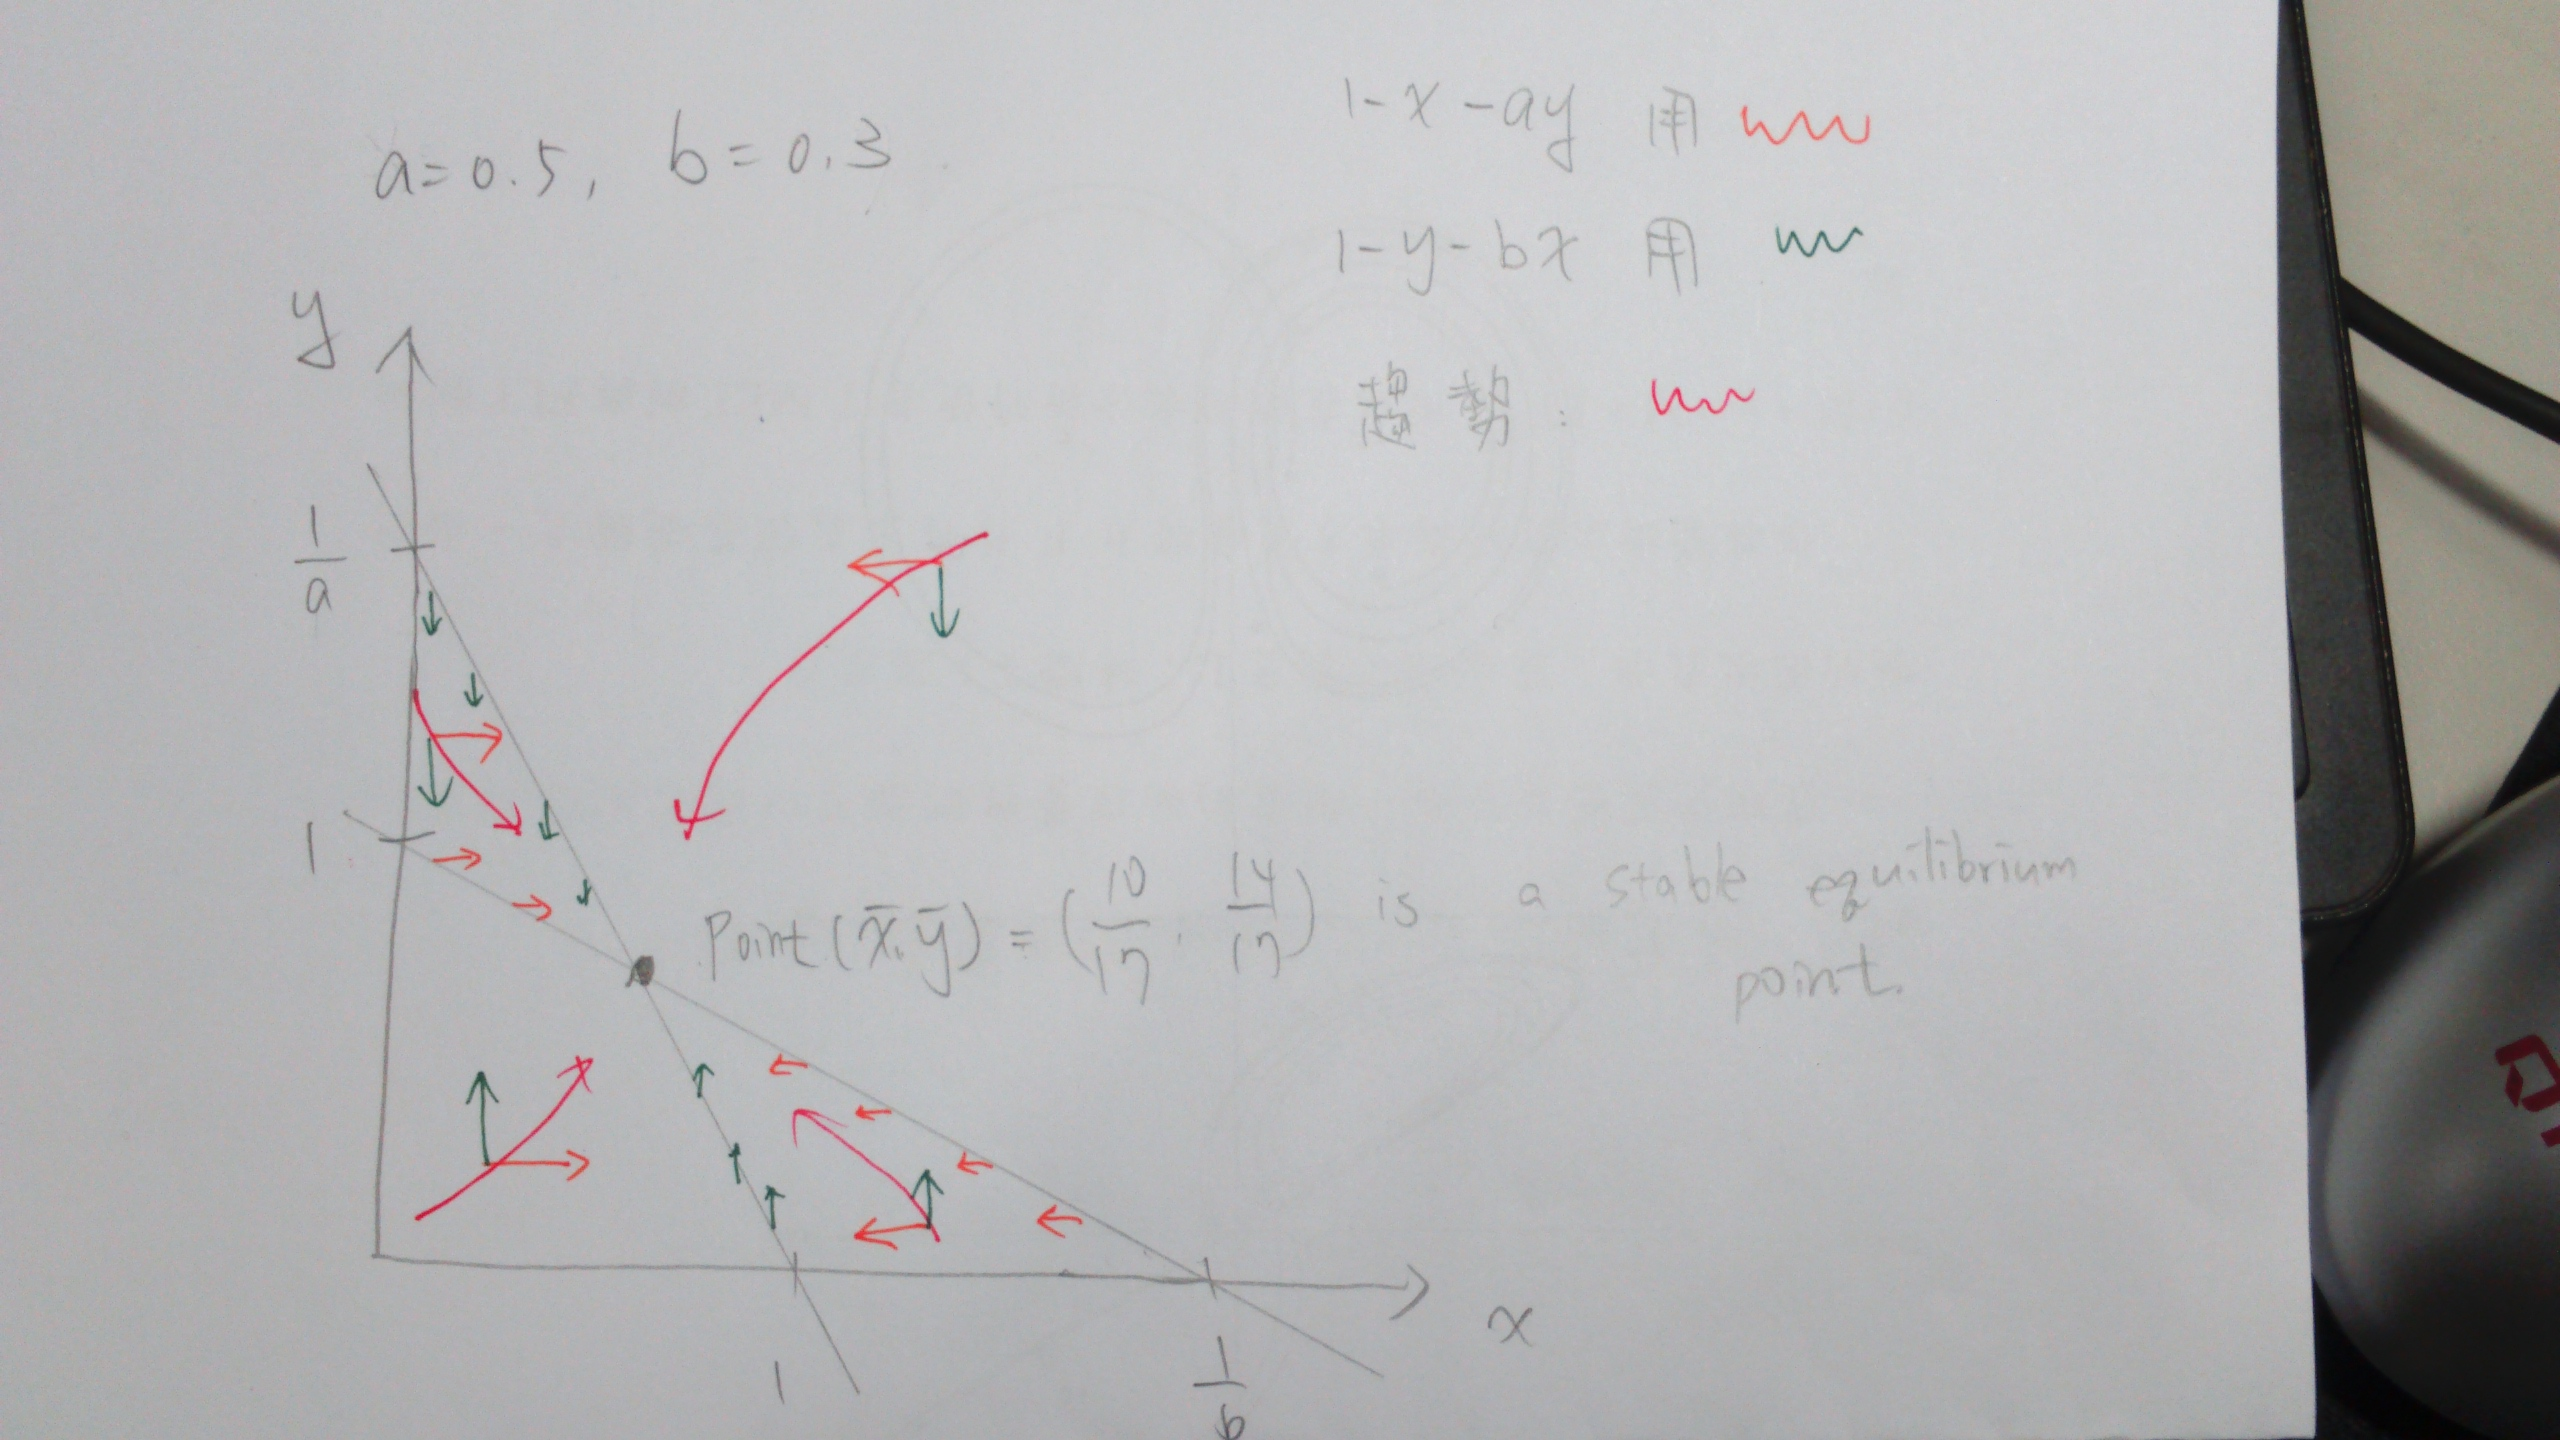
\includegraphics [width=\linewidth]{fig1}
	According to Q3, tr(A) = $\frac{0.5\alpha_1+0.7\alpha_2}{-0.85} < 0$ and det(A) = $\frac{0.35\alpha_1\alpha_2}{0.85} > 0$ (since $\alpha_1$ and $\alpha_2$ are $>$ 0), the point $(\overline{x}, \overline{y})$ is a stable equilibrium poing.

	\section {Problem 2}
	\subsection {Q1}
	Original equation:
	\[Gaussian = \frac{1}{\sqrt{2\sigma^2\pi}}e^{\frac{-(x-x_o)^2}{2\sigma^2}}\]
	Modified equation (by changing $\sigma$ to $\frac{\sigma}{3}$):
	\[Modified \;Gaussian = \frac{3}{\sqrt{2\sigma^2\pi}}e^{\frac{-9(x-x_o)^2}{2\sigma^2}}\]
	My thought is that the range is around from (0, 30) to (10, 20) (3 = $\frac{30-0}{20-10}$)
	\subsection {Q2}
	If using Delta func, we may set
	\[Delta \;func(x) = \left\{ \begin{array}{rcl} 0.2 & \mbox{for} & 12.5\leq x\leq17.5 \\
												0 & \mbox{for} & otherwise\end{array} \right.\]
	The probability of Delta func for each element in (12.5, 17.5) are equal. It implies that there couldn't be any data out of (12.5, 17.5) since the probability is 0.\\
	In Gaussian, there could exist data out of (12.5, 17.5) but the probability is very small. Besides, the probability of data in (12.5, 17.5) are not equal.
\end {document}
